\documentclass{standalone}
\usepackage{graphicx}	
\usepackage{amssymb, amsmath}
\usepackage{color}

\usepackage{tikz}
\usetikzlibrary{intersections, backgrounds, calc}

\definecolor{light}{RGB}{220, 188, 188}
\definecolor{mid}{RGB}{185, 124, 124}
\definecolor{dark}{RGB}{143, 39, 39}
\definecolor{highlight}{RGB}{180, 31, 180}
\definecolor{gray10}{gray}{0.1}
\definecolor{gray20}{gray}{0.2}
\definecolor{gray30}{gray}{0.3}
\definecolor{gray40}{gray}{0.4}
\definecolor{gray60}{gray}{0.6}
\definecolor{gray70}{gray}{0.7}
\definecolor{gray80}{gray}{0.8}
\definecolor{gray90}{gray}{0.9}
\definecolor{gray95}{gray}{0.95}

\newcommand*{\offset}{0.025}

\begin{document}

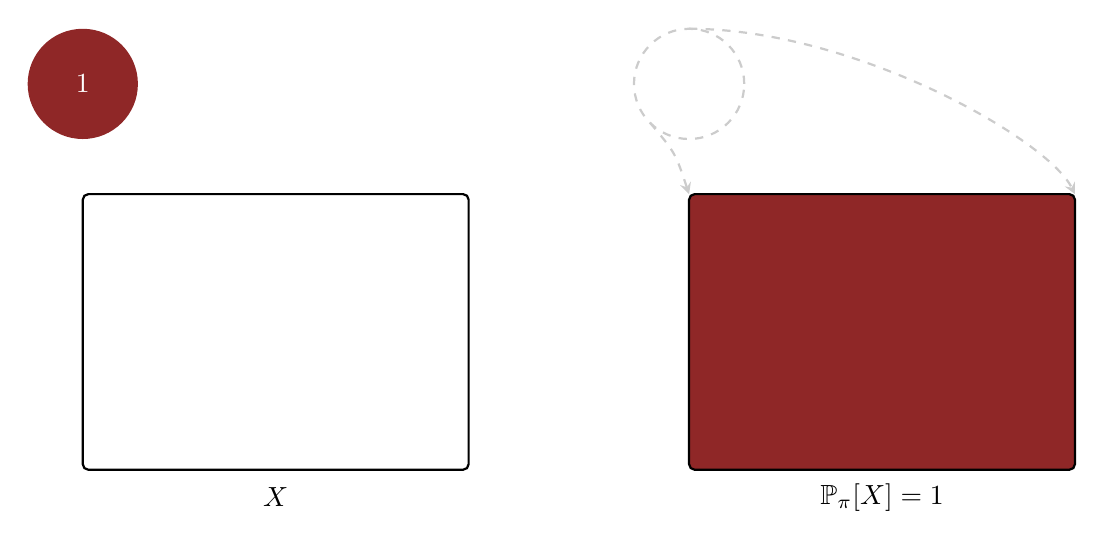
\begin{tikzpicture}[scale=0.35, thick]
  % Pre Distribution
  \draw [rounded corners=2pt, color=black] (-4, 0) rectangle +(-14, 10);
  \node at (-11, -1) { $X$ };
  
  \fill [color=dark, text=white] (-18, 14) circle (2) node {$1$}; 
  
  % Post Distribution
  \fill [rounded corners=2pt, color=dark] (4, 0) rectangle +(14, 10);

  \draw [rounded corners=2pt, color=black] (4, 0) rectangle +(14, 10);
  \node at (11, -1) { $\mathbb{P}_{\pi}[ X ] = 1$ };
  

  \draw [->, >=stealth, color=gray80, dashed] ({4 - sqrt(2)}, {14 - sqrt(2)}) .. controls (3.5, 11.5) .. (4, 10);
  \draw [->, >=stealth, color=gray80, dashed] (4, 16) .. controls (10, 16) and (17, 12) .. (18, 10);
    
  \draw [color=gray80, dashed] (4, 14) circle (2);
  
\end{tikzpicture}

\end{document}  